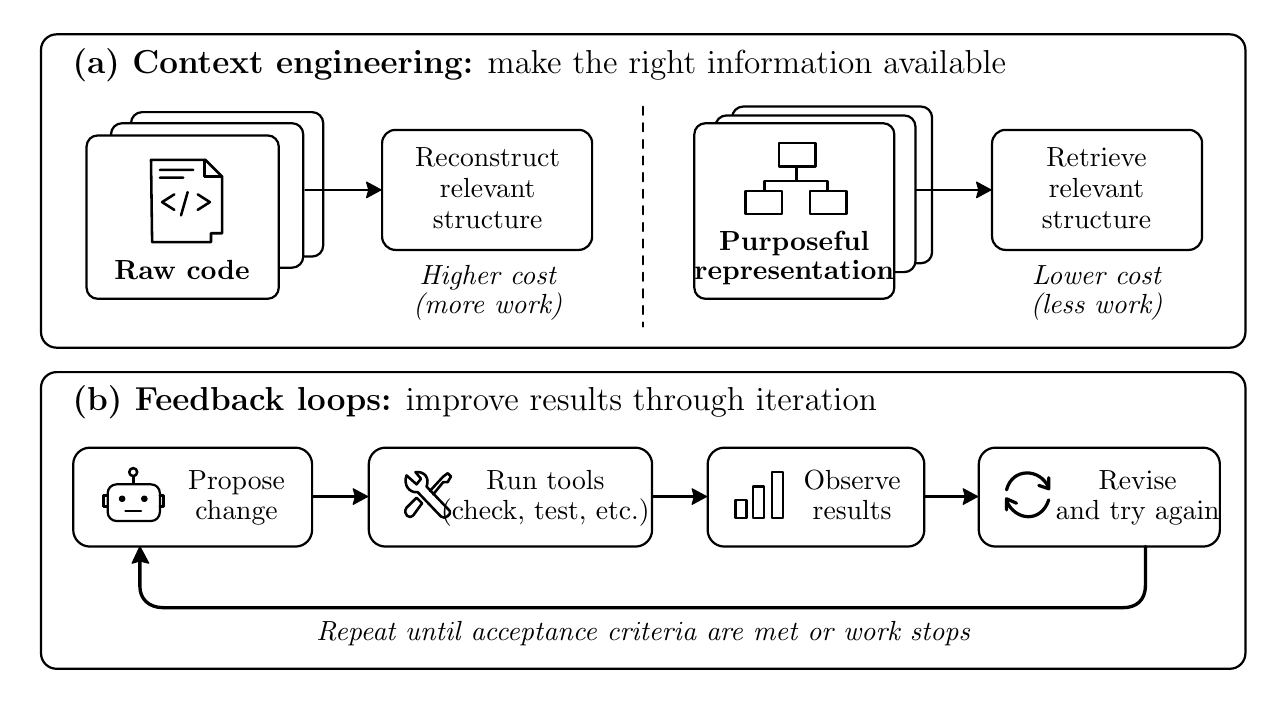
\begin{tikzpicture}[x=.4bp,y=-.4bp,line cap=round,line join=round]
\path[use as bounding box] (0,0) rectangle (1108,583);
\draw[rounded corners=5.6bp,line width=0.8bp,fill=white] (12,6) rectangle (1096,288);
\draw[rounded corners=5.6bp,line width=0.8bp,fill=white] (12,310) rectangle (1096,577);
\node[anchor=base west,inner sep=0pt,font=\magefigurefont\fontsize{12}{13}\selectfont] at (40,41) {\textbf{(a) Context engineering:} make the right information available};
\node[anchor=base west,inner sep=0pt,font=\magefigurefont\fontsize{12}{13}\selectfont] at (40,345) {\textbf{(b) Feedback loops:} improve results through iteration};
\draw[line width=0.72bp,dashed] (554,71) -- (554,269);
\draw[rounded corners=4bp,line width=0.8bp,fill=white] (93,76) rectangle (266,206);
\draw[rounded corners=4bp,line width=0.8bp,fill=white] (75,86) rectangle (248,216);
\draw[rounded corners=4bp,line width=0.8bp,fill=white] (53,97) rectangle (226,244);
\draw[rounded corners=4bp,line width=0.8bp,fill=white] (634,71) rectangle (814,212);
\draw[rounded corners=4bp,line width=0.8bp,fill=white] (619,79) rectangle (799,220);
\draw[rounded corners=4bp,line width=0.8bp,fill=white] (600,86) rectangle (780,244);
\draw[rounded corners=4.8bp,line width=0.8bp,fill=white] (319,92) rectangle (508,200);
\draw[rounded corners=4.8bp,line width=0.8bp,fill=white] (868,92) rectangle (1057,200);
\draw[line width=0.92bp] (250,146) -- (314,146);
\draw[line width=0.4bp,fill=black] (318,146) -- (305,139) -- (307,146) -- (305,153) -- cycle;
\draw[line width=0.92bp] (800,146) -- (863,146);
\draw[line width=0.4bp,fill=black] (867,146) -- (854,139) -- (856,146) -- (854,153) -- cycle;
\draw[line width=0.92bp] (112,193) -- (111,119) -- (160,119) -- (175,134) -- (175,185) -- (165,185) -- (165,193) -- cycle;
\draw[line width=0.92bp] (159,119) -- (159,134) -- (174,134);
\draw[line width=0.92bp] (119,128) -- (149,128) (119,135) -- (140,135) (132,150) -- (121,157) -- (132,164) (144,148) -- (138,169) (153,150) -- (164,157) -- (153,164);
\node[anchor=base,inner sep=0pt,outer sep=0pt,font=\magefigurefont\fontsize{10}{11.25}\selectfont\bfseries] at (139,227) {Raw code};
\draw[line width=0.92bp] (692,126) -- (692,137) (663,148) -- (663,138) -- (720,138) -- (720,148);
\draw[rounded corners=0bp,line width=0.8bp,fill=white] (676,104) rectangle (709,125);
\draw[rounded corners=0bp,line width=0.8bp,fill=white] (646,147) rectangle (679,168);
\draw[rounded corners=0bp,line width=0.8bp,fill=white] (704,147) rectangle (737,168);
\node[anchor=base,inner sep=0pt,outer sep=0pt,font=\magefigurefont\fontsize{9.6}{10.8}\selectfont\bfseries] at (690,201) {Purposeful};
\node[anchor=base,inner sep=0pt,outer sep=0pt,font=\magefigurefont\fontsize{9.6}{10.8}\selectfont\bfseries] at (690,227) {representation};
\node[anchor=base,inner sep=0pt,outer sep=0pt,font=\magefigurefont\fontsize{10}{11.25}\selectfont] at (414,125) {Reconstruct};
\node[anchor=base,inner sep=0pt,outer sep=0pt,font=\magefigurefont\fontsize{10}{11.25}\selectfont] at (414,153) {relevant};
\node[anchor=base,inner sep=0pt,outer sep=0pt,font=\magefigurefont\fontsize{10}{11.25}\selectfont] at (414,181) {structure};
\node[anchor=base,inner sep=0pt,outer sep=0pt,font=\magefigurefont\fontsize{10}{11.25}\selectfont\itshape] at (414,231) {Higher cost};
\node[anchor=base,inner sep=0pt,outer sep=0pt,font=\magefigurefont\fontsize{10}{11.25}\selectfont\itshape] at (414,257) {(more work)};
\node[anchor=base,inner sep=0pt,outer sep=0pt,font=\magefigurefont\fontsize{10}{11.25}\selectfont] at (962,125) {Retrieve};
\node[anchor=base,inner sep=0pt,outer sep=0pt,font=\magefigurefont\fontsize{10}{11.25}\selectfont] at (962,153) {relevant};
\node[anchor=base,inner sep=0pt,outer sep=0pt,font=\magefigurefont\fontsize{10}{11.25}\selectfont] at (962,181) {structure};
\node[anchor=base,inner sep=0pt,outer sep=0pt,font=\magefigurefont\fontsize{10}{11.25}\selectfont\itshape] at (962,231) {Lower cost};
\node[anchor=base,inner sep=0pt,outer sep=0pt,font=\magefigurefont\fontsize{10}{11.25}\selectfont\itshape] at (962,257) {(less work)};
\draw[rounded corners=6bp,line width=0.8bp,fill=white] (41,378) rectangle (256,467);
\draw[rounded corners=6bp,line width=0.8bp,fill=white] (307,378) rectangle (562,467);
\draw[rounded corners=6bp,line width=0.8bp,fill=white] (612,378) rectangle (807,467);
\draw[rounded corners=6bp,line width=0.8bp,fill=white] (856,378) rectangle (1073,467);
\draw[line width=0.92bp] (256,422) -- (302,422);
\draw[line width=0.4bp,fill=black] (306,422) -- (293,415) -- (295,422) -- (293,429) -- cycle;
\draw[line width=0.92bp] (562,422) -- (607,422);
\draw[line width=0.4bp,fill=black] (611,422) -- (598,415) -- (600,422) -- (598,429) -- cycle;
\draw[line width=0.92bp] (807,422) -- (851,422);
\draw[line width=0.4bp,fill=black] (855,422) -- (842,415) -- (844,422) -- (842,429) -- cycle;
\draw[rounded corners=3.2bp,line width=0.8bp,fill=white] (72,411) rectangle (119,444);
\draw[line width=.92bp,fill=white] (95,400) circle[radius=1.44bp];
\draw[line width=0.92bp] (95,404) -- (95,410) (72,421) -- (68,421) -- (68,431) -- (72,431) (119,421) -- (122,421) -- (122,431) -- (119,431);
\draw[line width=.92bp,fill=black] (85,424) circle[radius=0.72bp];
\draw[line width=.92bp,fill=black] (105,424) circle[radius=0.72bp];
\draw[line width=0.92bp] (88,435) -- (102,435);
\draw[line width=0.92bp] (341,403) .. controls (338,411) and (343,419) .. (351,418) -- (372,440) .. controls (375,443) and (382,438) .. (380,435) -- (359,413) .. controls (362,405) and (357,399) .. (349,400) -- (354,406) -- (350,411) -- cycle;
\draw[line width=0.92bp] (341,432) -- (350,423) -- (355,428) -- (347,439) .. controls (344,443) and (337,438) .. (341,432) -- cycle (362,417) -- (374,404) -- (378,401) -- (381,404) -- (378,409) -- (374,409) -- (365,420);
\draw[rounded corners=0bp,line width=0.8bp,fill=white] (637,425) rectangle (647,441);
\draw[rounded corners=0bp,line width=0.8bp,fill=white] (653,413) rectangle (663,441);
\draw[rounded corners=0bp,line width=0.8bp,fill=white] (670,400) rectangle (680,441);
\draw[line width=1.16bp] (881,416) .. controls (886,396) and (911,396) .. (919,414) (919,405) -- (919,415) -- (910,412) (919,425) .. controls (912,446) and (889,444) .. (881,426) (881,434) -- (881,424) -- (890,428);
\node[anchor=base,inner sep=0pt,outer sep=0pt,font=\magefigurefont\fontsize{9.6}{10.8}\selectfont] at (188,416) {Propose};
\node[anchor=base,inner sep=0pt,outer sep=0pt,font=\magefigurefont\fontsize{9.6}{10.8}\selectfont] at (188,443) {change};
\node[anchor=base,inner sep=0pt,outer sep=0pt,font=\magefigurefont\fontsize{9.6}{10.8}\selectfont] at (466,416) {Run tools};
\node[anchor=base,inner sep=0pt,outer sep=0pt,font=\magefigurefont\fontsize{9.6}{10.8}\selectfont] at (466,443) {(check, test, etc.)};
\node[anchor=base,inner sep=0pt,outer sep=0pt,font=\magefigurefont\fontsize{9.6}{10.8}\selectfont] at (742,416) {Observe};
\node[anchor=base,inner sep=0pt,outer sep=0pt,font=\magefigurefont\fontsize{9.6}{10.8}\selectfont] at (742,443) {results};
\node[anchor=base,inner sep=0pt,outer sep=0pt,font=\magefigurefont\fontsize{9.6}{10.8}\selectfont] at (999,416) {Revise};
\node[anchor=base,inner sep=0pt,outer sep=0pt,font=\magefigurefont\fontsize{9.6}{10.8}\selectfont] at (999,443) {and try again};
\draw[line width=1.2bp] (1006,467) -- (1006,502) .. controls (1006,516) and (997,522) .. (986,522) -- (122,522) .. controls (109,522) and (101,514) .. (101,503) -- (101,476);
\draw[line width=0.4bp,fill=black] (101,467) -- (94,482) -- (101,480) -- (109,482) -- cycle;
\node[anchor=base,inner sep=0pt,outer sep=0pt,font=\magefigurefont\fontsize{10}{11.25}\selectfont\itshape] at (554,552) {Repeat until acceptance criteria are met or work stops};
\end{tikzpicture}
